\subsection{MetaPredict}

Top scoring pairs is a robust algorithm for predicting gene expression profiles,
which adopts nonparametric rank-based prediction rule.
The MetaPredict is a meta-analysis version of the TSP algorithm that combines multiple transcriptomic studies to build a prediction model and shows improved 
prediction accuracy as compared to single study analysis.
The R package for MetaPredict module can be found \url{https://github.com/metaOmics/MetaPredict}.

The homepage for MetaPredict is shown in Figure \ref{fig:MetaPredictmainpage}.
Under advanced options,  there are 1 drop-down menu (``Methods for MetaPredict") {\color{red} (1)}, three number entries (``Max number of top scoring pairs (K)" {\color{red} (2)}, ``Number of cores for parallel computing" {\color{red} (3)}.
These will be introduced shortly but the users are not suggested to change them unless they know about the algorithm.
The necessay parameters include ``Number of top scoring pairs (K)" {\color{red} (7)}), three character entries (``Please select TWO labels to cluster" {\color{red} (4)}, ``Please select studies for training" {\color{red} (5)}, and ``Please select studies for testing") {\color{red} (6)} , and two excuting tabs ("Train model" and "Predict"). 

\subsubsection{Procedure}

\begin{figure}[H]
\begin{center}
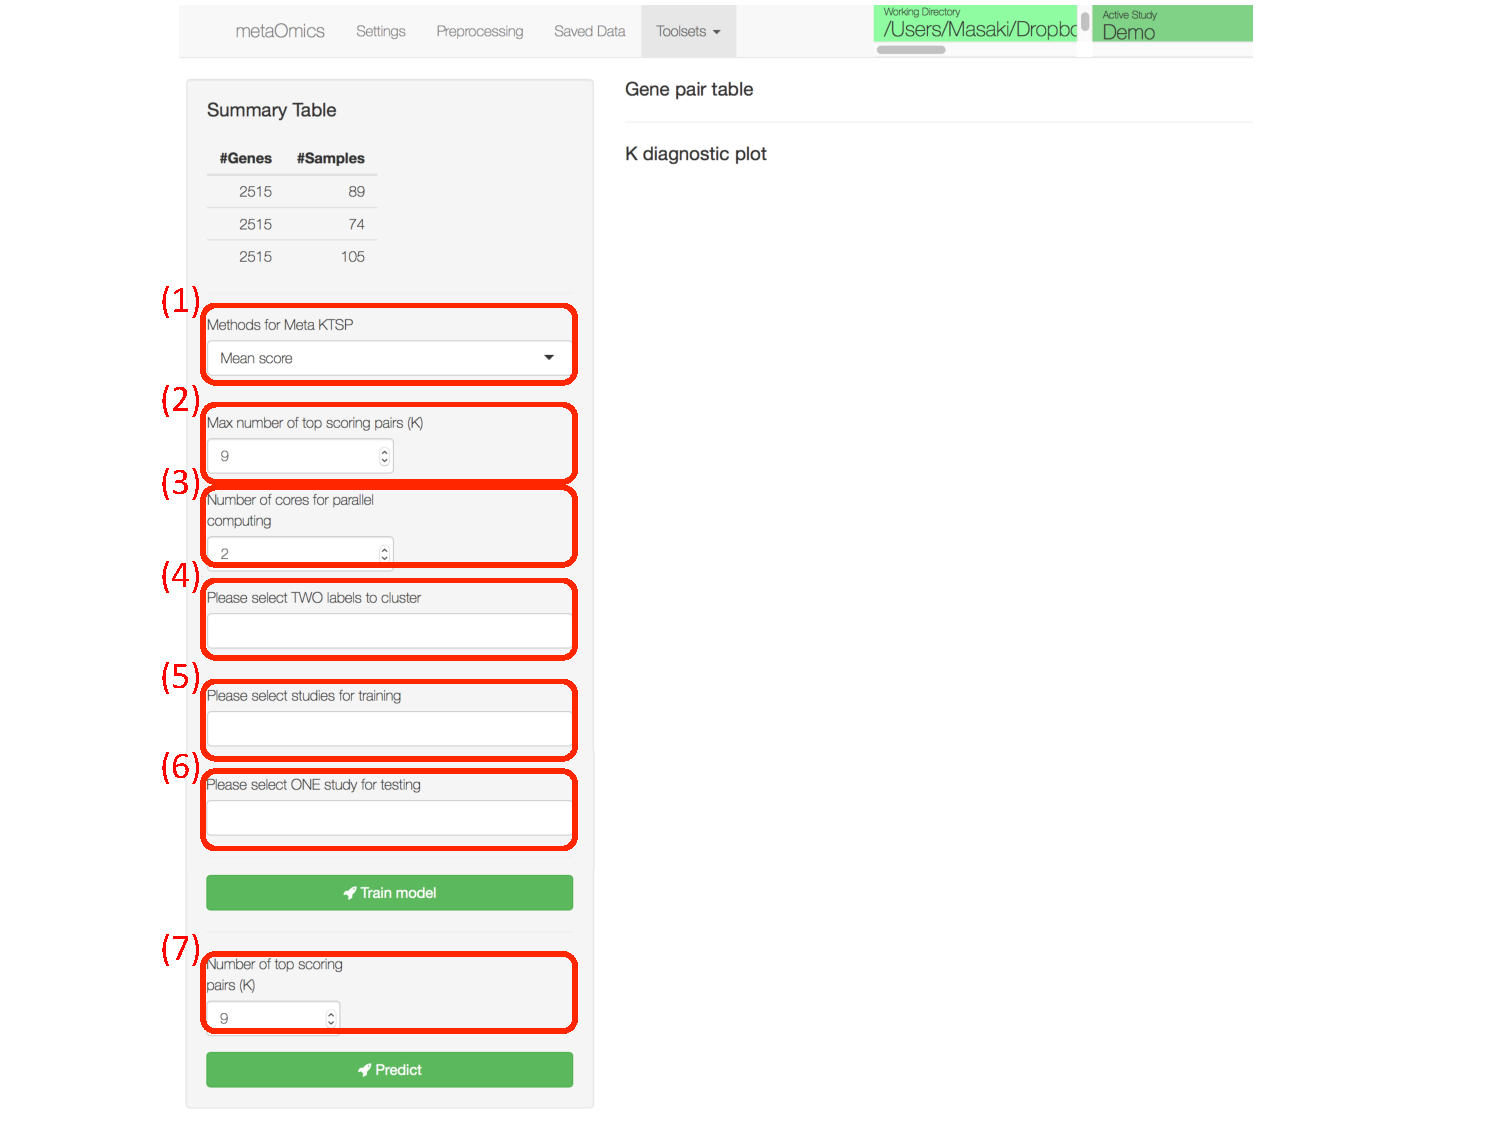
\includegraphics[scale=0.5]{./figure/MetaPredict/MetaPredictprocedure.pdf}
\caption{Homepage of MetaPredict}
\label{fig:MetaPredictmainpage}
\end{center}
\end{figure}

\begin{steps}
\item \textbf{Building prediction model based on meta-analysis}

First, we need to decide a method to select $K$ top scoring gene pairs from multiple studies (Figure \ref{fig:MetaPredictmainpage}). 
Second, we need to provide the maximum number of top scoring pairs $K$ (algorithm will search from 1 up to $K$ with default $K = 29$) and the number of cores for parallel computing. 
Next, we need to select only TWO labels to build the classification model. 
In other words, if there exists more than two kinds of labels, we need to choose two from them. 
If you click on {\color{red} (4)}, all available labels will pop up.
Then, select the dataset as training data and testing respectively, 
and click the "Train model" tab to run the MetaPredict program. 
It may take a while to run the model.

\item \textbf{MetaPredict prediction}

After the model training is finished, on the top right it will show up a ``Gene pair table" ({\color{red} (1)} in Figure \ref{fig:MetaPredictresult}) which present the top $K$ gene pairs statistics. 
A diagnostic plot ({\color{red} (2)} in Figure \ref{fig:MetaPredictresult}) is output to assist users decide which $K$ to use in the final prediction model. 
The suggested value is shown in the plot as green line, which is decided by VO method we introduced in the original paper. Users may also decide $K$ on their own to predict the class label of testing data. 
After deciding $K$, then hit the tab ``Predict'' (Figure \ref{fig:MetaPredictresult}). 
Finally, a confusion matrix is output to show the prediction results ({\color{red} (1)} in Figure \ref{fig:MetaPredictresult}).
The prediction results are also saved in the working direction.

\begin{figure}[H]
\begin{center}
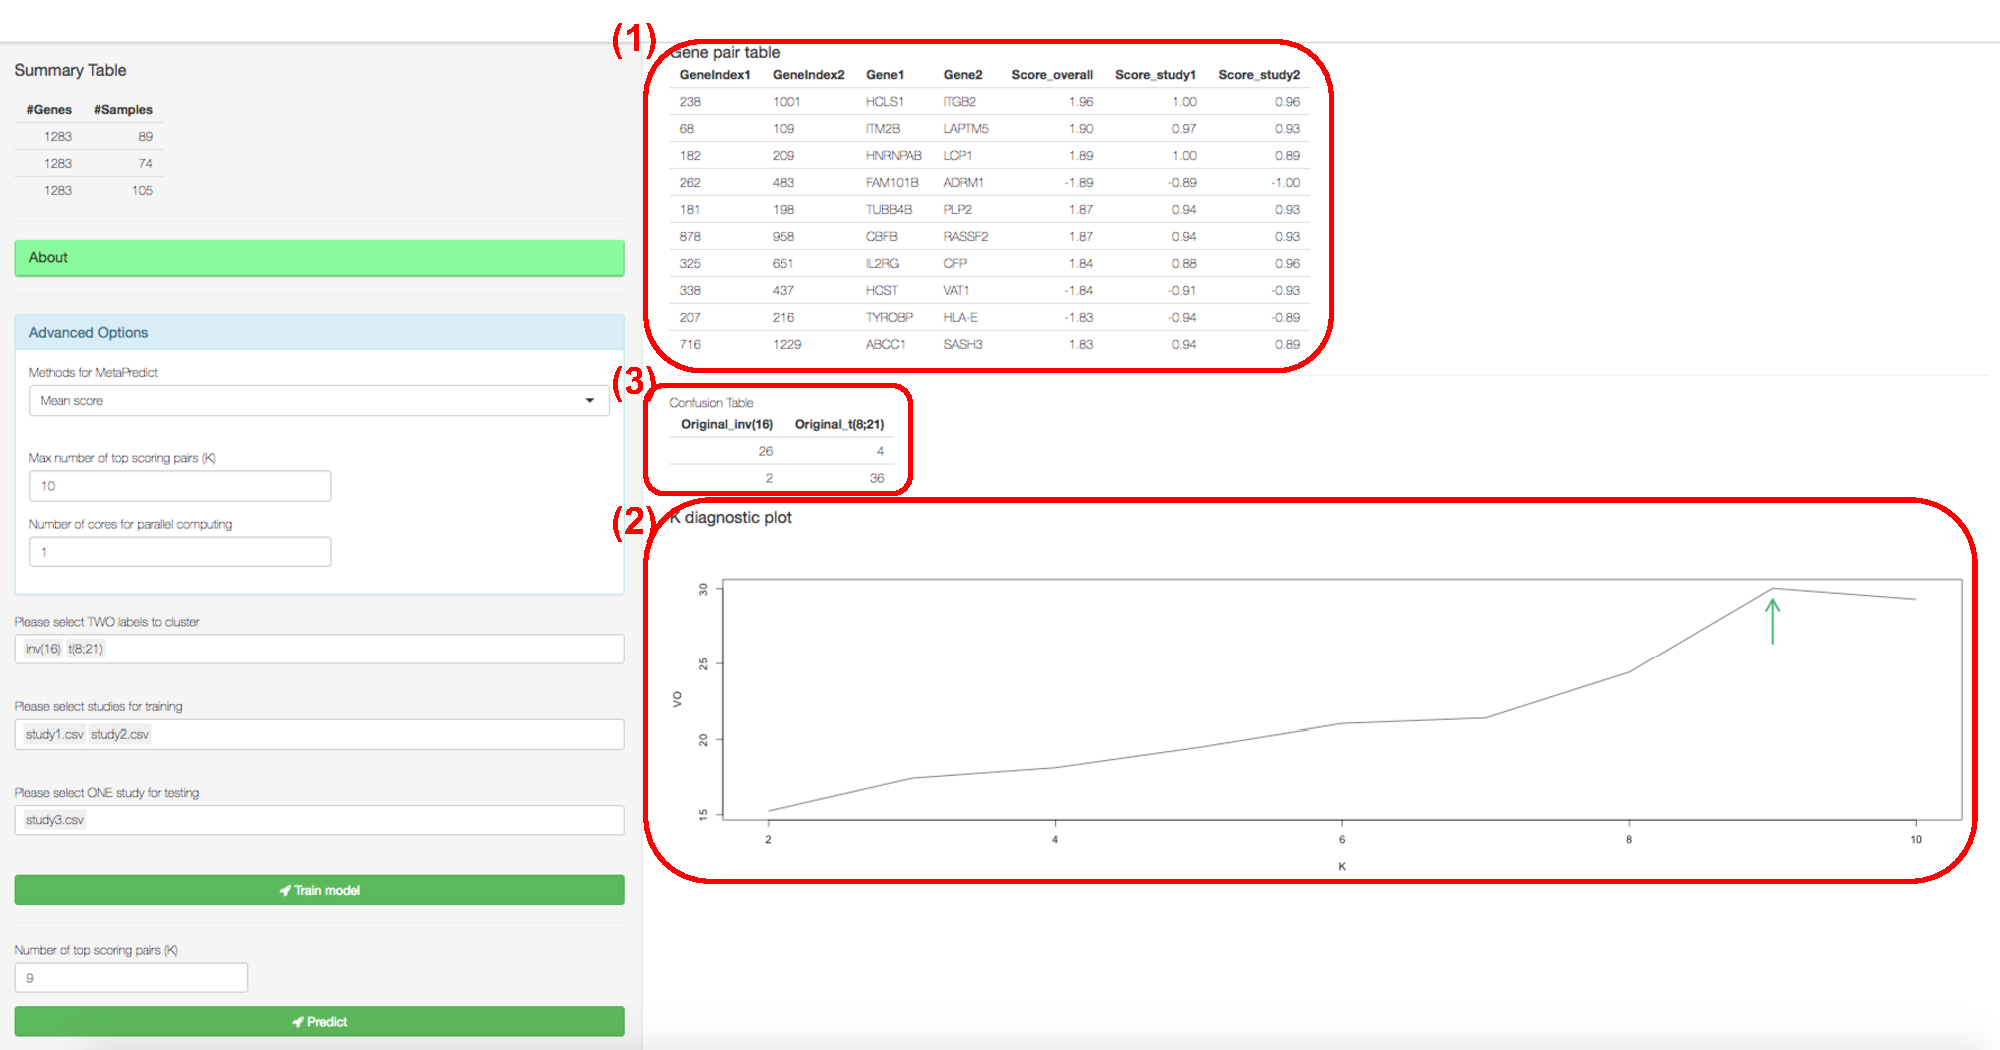
\includegraphics[scale=0.5]{./figure/MetaPredict/MetaPredictresult.pdf}
\caption{Results for MetaPredict.}
\label{fig:MetaPredictresult}
\end{center}
\end{figure}

\end{steps}

\textbf{Complete List of Options:} 
\begin{enumerate}
\item Model trainings: 
\begin{itemize}
\item Methods for MetaPredict: include Mean score, Fisher, Stouffer.
\item Max number of top scoring pairs (K)
\item Number of cores for parallel computing
\item TWO labels to cluster: labels for MetaPredict
\item Please select studies for training
\item Please select studies for testing
\item Number of top scoring pairs (K): Number of top scoring pairs (K) for prediction.
\end{itemize}

\end{enumerate}

\subsubsection{Results}

We used multi-study leukemia gene expression data as example.
After performing merging of the three datasets and filter 50\% genes by mean and 50\% by variance, 1283 genes remained.
In this example we only compare two phenotypes: inv(16) and t(8;21). 
Detailed descriptions of these studies can be found in Table~\ref{tab:realDataLeukemia}. 
A confusion matrix is output to show the prediction results ({\color{red} (1)} in Figure \ref{fig:MetaPredictresult}).
The prediction results are also saved in the working direction.

